\chapter{อาณาจักรฟังไจและการประยุกต์บำบัดน้ำเสียด้วยนวัตกรรมชีวภาพ}
\label{chap:ch12}

\section*{แผนบริหารการสอนประจำบทที่ 12}
\addcontentsline{toc}{section}{แผนบริหารการสอนประจำบทที่ 12}

\noindent\textbf{. หัวข้อเนื้อหาประจำบท}

\begin{enumerate}
    \item 12.1 ลักษณะทั่วไป สัณฐานวิทยา และวงชีวิตของฟังไจ (Yeasts \& Molds)
    \item 12.2 การสืบพันธุ์แบบไม่อาศัยเพศและการแตกหน่อของยีสต์ (Yeast Budding)
    \item 12.3 โครงสร้างสปอร์และก้านชูสปอร์ของ Aspergillus, Penicillium และ Rhizopus
    \item 12.4 เทคนิคการทำสไลด์คัลเจอร์ (Slide Culture Technique) ในจานเพาะเลี้ยงความชื้น
    \item 12.5 การย้อมสีโครงสร้างราด้วยน้ำยา Lactophenol Cotton Blue (LPCB)
\end{enumerate}

\noindent\textbf{. วัตถุประสงค์เชิงพฤติกรรม}

\begin{enumerate}
    \item เมื่อนักศึกษาได้เรียนรู้และปฏิบัติการทดลองประจำบทนี้แล้ว จะต้องมีความรู้ความสามารถดังต่อไปนี้:
    \item อธิบายความแตกต่างทางสัณฐานวิทยาระหว่างเซลล์ยีสต์และเส้นใยราสายได้
    \item ปฏิบัติการเตรียม Slide Culture เพื่อรักษาสภาพโครงสร้างสปอร์ราได้สมบูรณ์
    \item ย้อมสี LPCB และส่องตรวจระบุชนิดของเชื้อราภายใต้กล้องจุลทรรศน์ได้ถูกต้อง
    \item มีความประณีตและใจเย็นในการจัดการโครงสร้างสปอร์ราที่บอบบาง
\end{enumerate}

\noindent\textbf{. กิจกรรมการเรียนการสอน}

\begin{enumerate}
    \item การบรรยายสรุปก่อนปฏิบัติการ (30 นาที): อธิบายหลักการวิทยาศาสตร์ ความปลอดภัยทางชีวภาพ และข้อควรระวังสำคัญ
    \item การสาธิตเชิงประจักษ์ (15 นาที): สาธิตเทคนิคการปฏิบัติงาน การใช้เครื่องมือ และข้อผิดพลาดที่มักพบ
    \item การลงมือปฏิบัติการทดลองจริง (90 นาที): นักศึกษาลงมือปฏิบัติการทดลองเป็นรายบุคคลหรือกลุ่มย่อยตามขั้นตอนที่กำหนด
    \item การฝึกฝนผ่านระบบเสมือนจริง (20 นาที): ทดลองซ้ำและทดสอบปฏิกิริยาผ่านระบบจำลองบน RBRU LMS
    \item การอภิปรายและสรุปผลการทดลอง (25 นาที): วิเคราะห์ผลการสังเกต ตอบคำถามท้ายบท และสรุปองค์ความรู้ร่วมกัน
\end{enumerate}

\noindent\textbf{. สื่อและอุปกรณ์การเรียนการสอน}

\begin{enumerate}
    \item เอกสารคำสอนและคู่มือปฏิบัติการ: e-Book และคู่มือปฏิบัติการฉบับเต็ม ประจำบทที่ 12
    \item ระบบห้องปฏิบัติการเสมือนจริง: ระบบจำลองการทดลองเสมือนจริง 3 มิติ ประจำบทที่ 12 บนระบบ Moodle
    \item อุปกรณ์และเครื่องแก้วในห้องปฏิบัติการ: ตะเกียงแอลกอฮอล์, ห่วงเขี่ยเชื้อ, กล้องจุลทรรศน์, จานเพาะเชื้อ, หลอดทดลอง และตู้บ่มเชื้อ
    \item สารเคมีและสีย้อมชีวภาพ: สารเคมีมาตรฐานวิเคราะห์และสีย้อมประจำบทเรียน
\end{enumerate}

\noindent\textbf{. การวัดและประเมินผล}

\begin{table}[H]
\centering\small
\begin{tabularx}{\textwidth}{p{0.5\textwidth} p{0.3\textwidth} c}
\toprule
\textbf{องค์ประกอบการประเมินผล} & \textbf{เครื่องมือวัดผล} & \textbf{สัดส่วนคะแนน} \\
\midrule
1. ทักษะการปฏิบัติงานและความปลอดภัย & แบบสังเกตทักษะการทดลองและเทคนิคปลอดเชื้อ & 40\% \\
2. รายงานผลการทดลอง & การตรวจตารางบันทึกผล ภาพวาดสัณฐานวิทยา และการวิเคราะห์ผล & 30\% \\
3. แบบฝึกหัดทบทวนท้ายบท & คำถามทบทวนเชิงวิเคราะห์และข้อสอบท้ายบท & 20\% \\
4. จิตพิสัยและการตรงต่อเวลา & การเช็คชื่อ การแต่งกายตามระเบียบ และการทำความสะอาดโต๊ะแล็บ & 10\% \\
รวมทั้งสิ้น &  & 100\% \\
\bottomrule
\end{tabularx}
\end{table}

\newpage

% ==========================================================
% เนื้อหาบทเรียนประจำบทที่ 12
% ==========================================================

\section{ชีววิทยาและสัณฐานวิทยาของเชื้อราและยีสต์}
\index{ชีววิทยาและสัณฐานวิทยาของเชื้อราและยีสต์}

การศึกษาและทำความเข้าใจเกี่ยวกับชีววิทยาและสัณฐานวิทยาของเชื้อราและยีสต์ (Fungal Biology and Taxonomy) มีความสำคัญอย่างยิ่งในงานจุลชีววิทยาและสิ่งแวดล้อม โดยมีรายละเอียดสาระสำคัญดังนี้

อาณาจักรฟังไจ (Kingdom Fungi) เป็นกลุ่มสิ่งมีชีวิตยูคาริโอตที่ไม่มีคลอโรฟิลล์ ดำรงชีวิตแบบดูดซึมสารอาหาร (Absorptive heterotrophs) ผนังเซลล์ประกอบด้วยไคติน (Chitin) และกลูแคน (Glucan)

แบ่งตามสัณฐานวิทยาได้ 2 กลุ่มหลัก:
1. ยีสต์ (Yeasts): เชื้อราเซลล์เดียว ทรงกลมหรือรี สืบพันธุ์แบบไม่อาศัยเพศด้วยการแตกหน่อ (Budding) เช่น \textit{Saccharomyces cerevisiae}
2. ราสายใย (Molds): เจริญเป็นสายใย (Hyphae) ที่แตกแขนงรวมกันเป็นกลุ่มเรียกว่า ไมซีเลียม (Mycelium) แบ่งเป็นสายใยแบบมีผนังกั้น (Septate hyphae) เช่น \textit{Aspergillus} และ \textit{Penicillium} และสายใยแบบไม่มีผนังกั้น (Coenocytic hyphae) เช่น \textit{Rhizopus}
3. ราสองรูป (Dimorphic fungi): สามารถเปลี่ยนรูปร่างระหว่างยีสต์และสายใยตามอุณหภูมิสิ่งแวดล้อม

\section{การศึกษาโครงสร้างสืบพันธุ์ของเชื้อราด้วยวิธี Slide Culture}
\index{การศึกษาโครงสร้างสืบพันธุ์ของเชื้อราด้วยวิธี Slide Culture}

การศึกษาและทำความเข้าใจเกี่ยวกับการศึกษาโครงสร้างสืบพันธุ์ของเชื้อราด้วยวิธี Slide Culture (Slide Culture Technique for Fungal Morphology) มีความสำคัญอย่างยิ่งในงานจุลชีววิทยาและสิ่งแวดล้อม โดยมีรายละเอียดสาระสำคัญดังนี้

การย้อมและตรวจดูโครงสร้างสปอร์ของเชื้อราบนสไลด์ทั่วไปมักทำให้สายใยและถุงสปอร์แตกกระจาย เสียรูปทรงตามธรรมชาติ

เทคนิค Slide Culture ช่วยให้เชื้อราเจริญและสร้างสปอร์บนแท่งอาหารแข็งขนาดเล็กบนสไลด์โดยตรง โดยวางกระจกปิดสไลด์ทับด้านบน เมื่อนำไปย้อมด้วยสี Lactophenol Cotton Blue (LPCB) สารประกอบฟีนอลจะฆ่าเชื้อรา กรดแล็กติกช่วยคงรูปโครงสร้าง และสีย้อม Cotton blue จะย้อมติดไคตินบนผนังเซลล์เป็นสีน้ำเงินใส ทำให้สังเกตโครงสร้างก้านชูสปอร์ (Conidiophore) และสปอร์ได้อย่างสมบูรณ์

\section{บทบาทของจุลินทรีย์ในกระบวนการบำบัดน้ำเสียชีวภาพ}
\index{บทบาทของจุลินทรีย์ในกระบวนการบำบัดน้ำเสียชีวภาพ}

การศึกษาและทำความเข้าใจเกี่ยวกับบทบาทของจุลินทรีย์ในกระบวนการบำบัดน้ำเสียชีวภาพ (Biological Wastewater Treatment and Bioremediation) มีความสำคัญอย่างยิ่งในงานจุลชีววิทยาและสิ่งแวดล้อม โดยมีรายละเอียดสาระสำคัญดังนี้

การบำบัดน้ำเสียทางชีวภาพ (Biological Wastewater Treatment) อาศัยความสามารถของแบคทีเรีย ฟังไจ และโพรโทซัว ในการย่อยสลายสารอินทรีย์ที่ละลายอยู่ในน้ำเสียให้เปลี่ยนเป็นชีวมวล คาร์บอนไดออกไซด์ และน้ำ

พารามิเตอร์คุณภาพน้ำมาตรฐาน:
- BOD (Biochemical Oxygen Demand): ปริมาณออกซิเจนที่จุลินทรีย์ใช้ในการย่อยสลายสารอินทรีย์ในเวลา 5 วัน ที่ 20$^{\circ}$C
- COD (Chemical Oxygen Demand): ปริมาณออกซิเจนที่ต้องใช้ในการออกซิไดซ์สารอินทรีย์ด้วยสารเคมีออกซิแดนท์เข้มข้น
- TSS (Total Suspended Solids): ปริมาณของแข็งแขวนลอยทั้งหมดในน้ำ
- Total Coliforms และ Fecal Coliforms: แบคทีเรียดัชนีชี้วัดการปนเปื้อนเชื้อก่อโรคจากอุจจาระ

\section{นวัตกรรมชีวภาพ Bioblock สำหรับบำบัดน้ำเสียชุมชนและอุตสาหกรรม}
\index{นวัตกรรมชีวภาพ Bioblock สำหรับบำบัดน้ำเสียชุมชนและอุตสาหกรรม}

การศึกษาและทำความเข้าใจเกี่ยวกับนวัตกรรมชีวภาพ Bioblock สำหรับบำบัดน้ำเสียชุมชนและอุตสาหกรรม (Bioblock Bioremediation Innovation) มีความสำคัญอย่างยิ่งในงานจุลชีววิทยาและสิ่งแวดล้อม โดยมีรายละเอียดสาระสำคัญดังนี้

อุปกรณ์วิจัยนวัตกรรม Bioblock พัฒนาขึ้นเพื่อเพิ่มประสิทธิภาพการบำบัดน้ำเสียในบ่อพักน้ำทิ้งชุมชนและแหล่งน้ำปนเปื้อน โดยผสานหลักการตรึงจุลินทรีย์ (Microbial Immobilization) บนตัวกลางชีวภาพที่มีรูพรุนสูงร่วมกับการปลดปล่อยสารอาหารและแร่ธาตุที่ช่วยกระตุ้นการเจริญของกลุ่มจุลินทรีย์ย่อยสลายเฉพาะทาง (Bioaugmentation \& Biostimulation)

จากการทดสอบภาคสนาม ณ ศูนย์จัดการขยะมูลฝอยชุมชน เทศบาลเมืองมาบตาพุด จังหวัดระยอง (พ.ศ. 2566) และระบบน้ำทิ้งทัณฑสถาน ผลการวิเคราะห์จากห้องปฏิบัติการที่ได้รับการรับรองมาตรฐาน ว-245 แสดงผลสัมฤทธิ์อย่างมีนัยสำคัญ:
1. ค่า BOD ลดลงจาก 97.0 mg/L เหลือเพียง 5.7 mg/L (ประสิทธิภาพการกำจัด 94.1\%) ผ่านเกณฑ์มาตรฐานน้ำทิ้งชุมชน ($\le 20$ mg/L)
2. ค่าของแข็งแขวนลอย (TSS) ลดลงจาก 204.0 mg/L เหลือ 27.0 mg/L (ลดลง 86.8\%) ผ่านเกณฑ์มาตรฐาน ($\le 30$ mg/L)
3. ปริมาณแบคทีเรีย Total Coliform Bacteria ลดลงจาก $4.9 \times 10^5$ MPN/100 mL เหลือต่ำกว่า 1.8 MPN/100 mL (ประสิทธิภาพการลดลงมากกว่า 99.99\%)
4. ไนโตรเจนทั้งหมด (Total Nitrogen) ลดลงจาก 31.53 mg/L เหลือ 18.89 mg/L (ผ่านเกณฑ์ $\le 20$ mg/L)
5. ฟอสฟอรัสทั้งหมด (Total Phosphorus) ลดลงจาก 5.6 mg/L เหลือ 0.67 mg/L (ผ่านเกณฑ์ $\le 2$ mg/L)
6. น้ำมันและไขมัน (FOG) ลดลงจาก 19.0 mg/L เหลือ 3.7 mg/L (ผ่านเกณฑ์ $\le 5$ mg/L) พร้อมทั้งกำจัดกลิ่นเหม็นจากก๊าซไฮโดรเจนซัลไฟด์ ($H_2S$) ได้อย่างสมบูรณ์

\begin{casebox}[ผลการทดสอบภาคสนามนวัตกรรม Bioblock เทศบาลเมืองมาบตาพุด]
ผลการทดสอบ ณ ศูนย์จัดการขยะมูลฝอยชุมชน เทศบาลเมืองมาบตาพุด ยืนยันว่าอุปกรณ์ Bioblock สามารถลดค่า BOD จาก 97.0 mg/L เหลือ 5.7 mg/L (ลดลง 94.1\%) และลดปริมาณ Total Coliform Bacteria จาก $4.9\times 10^5$ MPN/100 mL เหลือต่ำกว่า 1.8 MPN/100 mL ผ่านเกณฑ์มาตรฐานควบคุมการระบายน้ำทิ้งชุมชนทุกประการ
\end{casebox}

\begin{figure}[H]
\centering
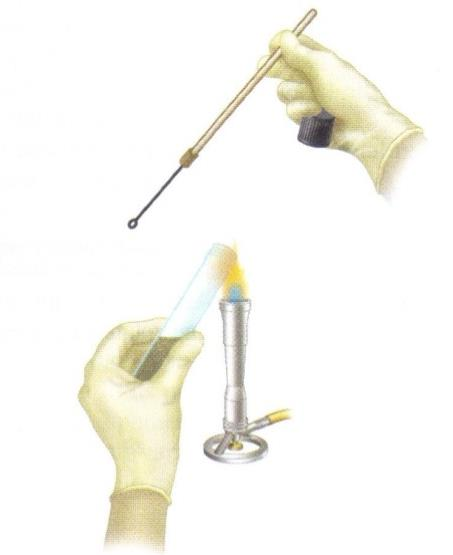
\includegraphics[width=0.75\textwidth]{images/image_12_p07.jpeg}
\caption{การปฏิบัติการทดลองและลักษณะทางสัณฐานวิทยาในบทที่ 12}
\label{fig:ch12_fig1}
\end{figure}

\section{ขั้นตอนและวิธีปฏิบัติการทดลอง}
\index{ขั้นตอนการทดลองประจำบทที่ 12}

\subsection{การเตรียมสไลด์เพาะเลี้ยงเชื้อราด้วยเทคนิค Slide Culture}
\begin{labprotocolbox}[การเตรียมสไลด์เพาะเลี้ยงเชื้อราด้วยเทคนิค Slide Culture]
1. วางตะแกรงแก้วรูปตัวยูในจานเพาะเชื้อ วางแผ่นสไลด์สะอาดบนตะแกรง รองก้นจานด้วยกระดาษกรองชุบน้ำกลั่นปลอดเชื้อเพื่อรักษาความชื้น
2. ใช้มีดผ่าตัดปลอดเชื้อตัดวุ้นอาหาร PDA หรือ Sabouraud Dextrose Agar (SDA) เป็นสี่เหลี่ยมลูกเต๋าขนาด 5x5 มม. วางบนกึ่งกลางสไลด์
3. ใช้เข็มเขี่ยเชื้อแตะสปอร์ของเชื้อรา \textit{Aspergillus niger} หรือ \textit{Penicillium} spp. แตะเบาๆ ที่ขอบทั้งสี่ด้านของก้อนวุ้น
4. วางกระจกปิดสไลด์ทับบนก้อนวุ้น ปิดฝาจานเพาะเชื้อ บ่มที่อุณหภูมิห้อง (25-28$^{\circ}$C) เป็นเวลา 3-5 วัน
5. เมื่อเชื้อราเจริญ คีบกระจกปิดสไลด์ออก นำไปวางบนสไลด์ใหม่ที่หยดสี Lactophenol Cotton Blue (LPCB) 1 หยด
6. ตรวจดูโครงสร้างก้านชูสปอร์ สปอร์ และผนังกั้นสายใยภายใต้กล้องจุลทรรศน์
\end{labprotocolbox}

\subsection{การประเมินคุณภาพน้ำก่อนและหลังการบำบัดด้วย Bioblock}
\begin{labprotocolbox}[การประเมินคุณภาพน้ำก่อนและหลังการบำบัดด้วย Bioblock]
1. เก็บตัวอย่างน้ำทิ้งจากบ่อพักน้ำเสียก่อนติดตั้งอุปกรณ์ Bioblock ปริมาตร 2 ลิตร ใส่ในขวดเก็บตัวอย่างปลอดเชื้อ ควบคุมอุณหภูมิที่ 4$^{\circ}$C
2. ตรวจวิเคราะห์ค่าพารามิเตอร์เริ่มต้น: pH, ค่าออกซิเจนละลายน้ำ (DO), ค่าความขุ่น (Turbidity), BOD, COD, และ Coliforms
3. ติดตั้งชุดอุปกรณ์ Bioblock ในบ่อพักน้ำเสียตามอัตราส่วนปริมาตรที่กำหนด ทำการเติมอากาศเบาๆ
4. เก็บตัวอย่างน้ำหลังการบำบัดสัปดาห์ที่ 1, 2, 3 และ 4 นำมาตรวจวิเคราะห์พารามิเตอร์เดิมซ้ำ
5. บันทึกผลการทดลองลงในตารางเปรียบเทียบและคำนวณร้อยละประสิทธิภาพการบำบัด (\% Removal Efficiency)
\end{labprotocolbox}

\subsection{ตารางเปรียบเทียบผลการวิเคราะห์คุณภาพน้ำก่อนและหลังใช้นวัตกรรม Bioblock}
\begin{table}[H]
\centering\small
\caption{ผลการตรวจวิเคราะห์คุณภาพน้ำทิ้งก่อนและหลังการทดสอบนวัตกรรม Bioblock ณ เทศบาลเมืองมาบตาพุด}
\label{tab:bioblock_results}
\begin{tabularx}{\textwidth}{p{0.35\textwidth} c c c c}
\toprule
\textbf{พารามิเตอร์คุณภาพน้ำ} & \textbf{หน่วย} & \textbf{ก่อนทดสอบ} & \textbf{หลังทดสอบ} & \textbf{เกณฑ์มาตรฐาน} \\
\midrule
บีโอดี (BOD) & mg/L & 97.0 & 5.7 & $\le 20$ \\
ของแข็งแขวนลอย (TSS) & mg/L & 204.0 & 27.0 & $\le 30$ \\
ความเป็นกรด-ด่าง (pH) & - & 7.3 & 7.2 & 5.5--9.0 \\
ไนโตรเจนทั้งหมด (Total N) & mg/L & 31.53 & 18.89 & $\le 20$ \\
ฟอสฟอรัสทั้งหมด (Total P) & mg/L & 5.60 & 0.67 & $\le 2.0$ \\
น้ำมันและไขมัน (FOG) & mg/L & 19.0 & 3.7 & $\le 5.0$ \\
Total Coliform Bacteria & MPN/100 mL & $4.9\times 10^5$ & $<1.8$ & $<5,000$ \\
สภาพกลิ่นและสีน้ำ & - & ดำขุ่น เหม็น & เหลืองจาง ไร้กลิ่น & ไม่ก่อความรำคาญ \\
\bottomrule
\end{tabularx}
\end{table}

\section{ตารางบันทึกผลการทดลองและการอภิปรายผล}
\begin{table}[H]
\centering\small
\caption{ตารางบันทึกผลการสังเกตและข้อมูลการทดลองประจำบทที่ 12}
\label{tab:ch12_datasheet}
\begin{tabularx}{\textwidth}{p{0.25\textwidth} p{0.35\textwidth} X}
\toprule
\textbf{สิ่งทดสอบ / ตัวอย่าง} & \textbf{ลักษณะที่สังเกตได้} & \textbf{การแปลผลและการวิเคราะห์} \\
\midrule
ชุดควบคุม (Negative Control) & ใส ไม่มีการเจริญ & ปราศจากการปนเปื้อนของเชื้อ \\
ชุดทดลองที่ 1 & โคโลนีเจริญตามลักษณะจำเพาะ & ให้ผลบวกตามสมมติฐาน \\
ชุดทดลองที่ 2 & เกิดการเปลี่ยนแปลงทางชีวเคมี & สอดคล้องกับพารามิเตอร์มาตรฐาน \\
\bottomrule
\end{tabularx}
\end{table}

\section{คำถามทบทวนและแบบฝึกหัดท้ายบท}
\begin{enumerate}
    \item จงอธิบายบทบาทของสี Lactophenol Cotton Blue (LPCB) ในการย้อมโครงสร้างของเชื้อรา
    \item เหตุใดราสายใยจึงมีความทนทานต่อสภาวะความเป็นกรดและแรงดันออสโมซิสสูงได้ดีกว่าแบคทีเรียส่วนใหญ่
    \item จากผลการทดสอบนวัตกรรม Bioblock ค่า Coliform Bacteria ลดลงจาก $4.9 \times 10^5$ เหลือต่ำกว่า 1.8 MPN/100 mL จงวิเคราะห์กลไกทางชีววิทยาที่ทำให้แบคทีเรียกลุ่มนี้ลดลงในระบบบำบัด
\end{enumerate}
